115. а) $$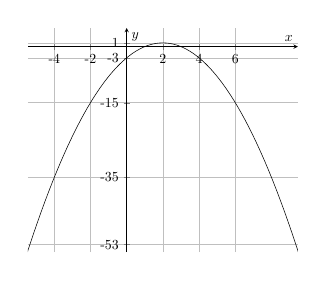
\begin{tikzpicture}[scale=0.5]
\begin{axis}[
    axis lines = middle,
    grid=major,
    legend pos={south west},
    xlabel = {$x$},
    ylabel = {$y$},
    ymin=-55,
    ymax=5,
    xtick={-6,-4,-2, 2,4,6,10},
    xticklabels={-6,-4,-2, 2,4,6,10},
    ytick={-53,-35,-15,1,-3},
    yticklabels={-53,-35,-15,1,-3}            ]
\addplot[domain=-8:10, samples=100, color=black] {-x*x+4*x-3};
\end{axis}
\end{tikzpicture}$$\\
б) $$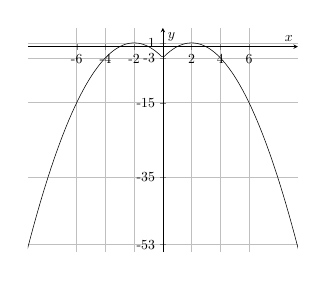
\begin{tikzpicture}[scale=0.5]
\begin{axis}[
    axis lines = middle,
    grid=major,
    legend pos={south west},
    xlabel = {$x$},
    ylabel = {$y$},
    ymin=-55,
    ymax=5,
    xtick={-6,-4,-2, 2,4,6,10},
    xticklabels={-6,-4,-2, 2,4,6,10},
    ytick={-53,-35,-15,1,-3},
    yticklabels={-53,-35,-15,1,-3}            ]
\addplot[domain=-10:10, samples=100, color=black] {-x*x+4*abs(x)-3};
\end{axis}
\end{tikzpicture}$$\\
